\section{Digital Microfluidics (DMF)}
Digital microfluidics (DMF) represents a significant departure from traditional microfluidic techniques. Instead of relying on continuous flow through intricate channel geometries and external micropumps, DMF controls liquid movement by manipulating individual droplets on a planar surface using localized electric fields applied on an array of electrodes \cite{abdelgawadDigitalRevolutionNew2009,fairChemicalBiologicalApplications2007}.\\

Due to smaller form factor, DMF allows smaller liquid volume for laboratory processes to be in microliter (\textmugreek L) and picoliter (pL), thus reducing reagents and samples wastage \cite{bhattacharjeeDropletPositionControl2010,royNewSamplePreparation2015}.\\

Another advantage of DMF have over microfluidics are reduced sample cross-contamination and dispersion. This is due to the droplet served as a self-contained microreactor, there is negligible cross-mixing between different samples or reagents \cite{luoMachineVisionbasedDriving2021,wuResearchProgressElectrode2023}.\newpage

\subsection{Architecture}
DMF are categorically divided into two configurations, which are open and closed as illustrated in Figure \ref{DMFConfig}.\\
\begin{figure}[h!]
    \centering
    \begin{subfigure}{0.45\textwidth}
        \centering
        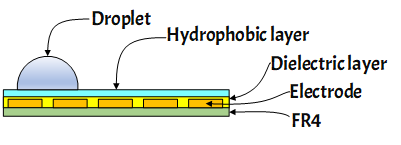
\includegraphics[width=\textwidth]{Open_TypeDMF.png}
        \caption{Open type DMF}
        \label{OpenTypeDMF}
    \end{subfigure}
    \begin{subfigure}{0.45\textwidth}
        \centering
        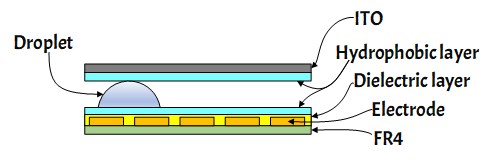
\includegraphics[width=\textwidth]{Closed_TypeDMF.png}
        \caption{Closed type DMF}
        \label{ClosedTypeDMF}
    \end{subfigure}
    \caption{Types of DMF configurations using FR4 as the substrate}
    \label{DMFConfig}
\end{figure}

Open-configuration DMF constitutes of a substrate where an array of electrodes (actuation and grounding connections included), a layer of dielectric layer and a layer of hydrophobic layer are deposited on top of it. Grounding methods for open-type DMF exhibit greater variability and may include a conductive probe inserted into the droplet, exposed ground traces interspersed between actuation electrodes, or subsurface grounding electrodes embedded below the dielectric layer \cite{yafiaDigitalMicrofluidicSystems2018}. The absence of an upper confining substrate results in the droplet interface being exposed to ambient conditions or, in certain implementations, immersed in a continuous oil phase to suppress evaporation and enhance droplet stability \cite{vafaieNumericalSimulationEWOD2019,yafiaHighPrecisionControl2013,yafiaLowCostGrapheneBasedDigital2020}. \\

The dielectric layer electrically isolates the actuating electrode array, thereby suppressing leakage currents and inhibiting electrolysis. A hydrophobic coating is deposited atop the dielectric to lower the surface energy and minimize droplet pinning \cite{abdelgawadDigitalRevolutionNew2009,agarwalDigitalMicrofluidicsTechniques2012,barmanElectrowettingondielectricEWODCurrent2020,jebrailLetsGetDigital2010}. Droplet actuation and transport are achieved through modulation of the interfacial forces under an applied electric field.\\

In the closed configuration, droplets are confined within the gap between two parallel substrates \cite{abdelgawadOptimizationDeviceGeometry2009,al-lababidiMinimumMovableDroplet2023}. The lower substrate incorporates a patterned electrode array for actuation, while the upper substrate—typically a continuous ground plane—is often fabricated from a transparent conductive material such as Indium Tin Oxide (ITO) to enable optical observation \cite{barmanElectrowettingondielectricEWODCurrent2020,sukthangRapidFabricationCloseTyped2020}. \\

Both the actuation electrodes on the bottom substrate and, in many cases, the ground electrode on the top substrate are coated with a dielectric layer to isolate the droplet and preventing electrolysis and dielectric breakdown. A hydrophobic coating is further applied to both surfaces to reduce contact angle hysteresis and enhance droplet mobility \cite{agarwalDigitalMicrofluidicsTechniques2012,jebrailDigitalMicrofluidicsVersatile2012,meimandiDevelopmentElectrowettingDigital2019}.\newpage

\subsection{Droplet Manipulation Techniques}

\subsection{Core Operations}
Generally, key droplet operations that can be executed by DMF are shown in Figure \ref{DMFOps} \cite{bhattacharjeeMultipleDilutionSample2012,bhattacharjeeEfficientGenerationDilution2019,bhattacharyaAlgorithmicChallengesDigital2014}.
\begin{figure}[h!]
    \smartdiagramset{bubble node font=\sffamily\large,
    bubble center node font=\sffamily\Huge}
    \centering
    \smartdiagram[bubble diagram]{
        DMF\\Operations,
        Transport,
        Merging,
        Splitting,
        Dispensing,
        Mixing,
        Storage,
        Sensing
        }
    \caption{DMF key operations}
    \label{DMFOps}
\end{figure}
